\documentclass[11pt]{article}
\usepackage{setspace}
\setstretch{1}
\usepackage[T1]{fontenc}
\usepackage{amsmath,amssymb, amsthm}
\usepackage{graphicx}
\usepackage{bm}
\usepackage[hang, flushmargin]{footmisc}
\usepackage[colorlinks=true]{hyperref}
\usepackage[nameinlink]{cleveref}
\usepackage{footnotebackref}
\usepackage{url}
\usepackage{listings}
\usepackage[most]{tcolorbox}
\usepackage{inconsolata}
\usepackage[papersize={8.5in,11in}, margin=1in]{geometry}
\usepackage{float}
\usepackage{caption}
\usepackage{esint}
\usepackage{url}
\usepackage{enumitem}
\usepackage{subfig}
\usepackage{wasysym}
\newcommand{\ilc}{\texttt}
\usepackage{etoolbox}
\usepackage{algorithm}
% \usepackage{algorithmic}
\usepackage[noend]{algpseudocode}
\usepackage{tikz}
\usetikzlibrary{matrix,positioning,arrows.meta,arrows}
\patchcmd{\thebibliography}{\section*{\refname}}{}{}{}

\makeatletter
\renewcommand{\@seccntformat}[1]{}
\makeatother


\begin{document}



\title{\textbf{EECS 340: Assignment 7}}

\author{Shaochen (Henry) ZHONG, \ilc{sxz517} \\ Yuhui ZHANG, \ilc{yxz2052}}
\date{Due and submitted on 04/27/2020 \\ EECS 340, Dr. Koyut{\"u}rk}
\maketitle

% % % % % % % % % % % % % % % % % % % % % % % % % % % % % % % % % %
% % % % % % % % % % % % % % % % % % % % % % % % % % % % % % % % % %
% % % % % % % % % % % % % % % % % % % % % % % % % % % % % % % % % %
\section{Problem 1}

% % % % % % % % % % % % % % % % % % % % % % % % % % % % % % % % % %
% % % % % % % % % % % % % % % % % % % % % % % % % % % % % % % % % %
\subsection{(a)}

Set the each team as a node (vertex) in graph $G$ and make every node fully connected (representing the fact that all teams have played against each other). If one team $A$ beats another team $B$, we will have a directed edge of $A \rightarrow B$ betwen the nodes representing $A$ and $B$.

\begin{algorithm}[H]
\caption{DFS(G)}
    \begin{algorithmic}[1]
        \Procedure{DFS}{G}
        \For{each $u \in G.V$}:
            \State $u.color$ = WHITE
            \State $u.z$ = 0
        \EndFor
        \For{each $u \in G.V$}:
            \If{$u.color$ == WHITE}
                \State \textsc{DFS-Game-Visit(G, u)}
            \EndIf
        \EndFor
    \end{algorithmic}
\end{algorithm}

\begin{algorithm}[H]
\caption{DFS-Game-Visit(G, u)}
    \begin{algorithmic}[1]
        \Procedure{DFS-Game-Visit}{G, u}
        \State $z = NULL$
        \State $u.color$ = GRAY
        \For{each $v \in Adj(u)$}:
            \If{$v.color$ == WHITE}
                \State $z = v.rank$
                \State $z = \min(z, \textsc{DFS-Game-Visit(G, v)})$
            \EndIf
        \EndFor
        \State $u.color$ = BLACK
        \If{$z == NULL$}
            \State $u.z = 0$
            \State $z = u.rank$
        \Else
            \State $u.z = z$
        \EndIf
        \State \Return $z$
    \end{algorithmic}
\end{algorithm}

% % % % % % % % % % % % % % % % % % % % % % % % % % % % % % % % % %
% % % % % % % % % % % % % % % % % % % % % % % % % % % % % % % % % %
\subsection{(b)}

\paragraph{Justification for runtime} The algorithm is $O(m+n)$ as DFS will first traverse every node, which means it will at least be $O(n)$. In addition, since the graph $G$ is implemented using adjacency list, for each node we will have to traverse through all its adjacent edges -- where such number can be at most $m$ (total number of edges in $G$) for a single node. Thus, the total time complexity is $O(m + n)$.

\paragraph{Justification for correctness} The algorithm basically performs a DFS travesal on the graph $G$ and set the node \ilc{u} with smallest \ilc{rank} value as \ilc{z} to all of node \ilc{u}'s ancestor nodes. Due to the nature of DFS, node \ilc{u}'s ancestor nodes can legally have \ilc{u.rank} as their domination factor, as being \ilc{u}'s ancestors imply the fact these teams have won against team \ilc{u}. Also in \texsc{DFS-Game-Visit} we will not set a node's \ilc{.z} value unless such node is marked as \ilc{BLACK} (which means all of its decedents have been explored). Combine these two observations, each node has explored all of its decendents nodes, and the node's decendent node with the smallest \ilc{rank} will be assigned as all its ancestor nodes' \ilc{.z} value. The algorithm is a perfect mimic of the game logic of domination factor and guaranteed to be correct.


% % % % % % % % % % % % % % % % % % % % % % % % % % % % % % % % % %
% % % % % % % % % % % % % % % % % % % % % % % % % % % % % % % % % %
% % % % % % % % % % % % % % % % % % % % % % % % % % % % % % % % % %
\section{Problem 2}

\subsection{(a)}

Disprove with conterexample:

\begin{figure}[H]
    \centering
    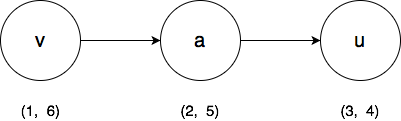
\includegraphics[width=0.6\linewidth]{{fig/fig_2_a.png}}
\end{figure}

Note the tuple below each node represents their \ilc{(start-time, finish-time)}. It is shown that $v.f > u.f$ as $6 > 4$, however there is no circle between $uv$. Thus, this conterexample disproves the statement.

% % % % % % % % % % % % % % % % % % % % % % % % % % % % % % % % % %
% % % % % % % % % % % % % % % % % % % % % % % % % % % % % % % % % %
% % % % % % % % % % % % % % % % % % % % % % % % % % % % % % % % % %
\section{Problem 4}

% \section{References}
%
% \nocite{*}
% \raggedright
% \bibliography{references.bib}
% \bibliographystyle{plain}


\end{document}